
\documentclass[letterpaper,hide notes,xcolor={table,svgnames},pdftex,10pt]{beamer}
\def\showexamples{t}

\usecolortheme{crane}
\setbeamertemplate{navigation symbols}{}

\usetheme{MyPittsburgh}
\usepackage{hyperref}
\usepackage{graphicx,xspace}
\usepackage[normalem]{ulem}
\usepackage{multicol}
\usepackage{amsmath,amssymb,amsthm,graphicx,xspace}
\newcommand\SF[1]{$\bigstar$\footnote{SF: #1}}

\usepackage{csquotes}
\renewcommand{\mkbegdispquote}[2]{\itshape}

\usepackage[sfdefault,lf]{carlito}
\usepackage[T1]{fontenc}
\usepackage[scaled]{beramono}
\usepackage{tikzpagenodes}
\newcommand{\Rplus}{\protect\hspace{-.1em}\protect\raisebox{.35ex}{\small{\small\textbf{+}}}}
\newcommand{\Cpp}{\mbox{C\Rplus\Rplus}\xspace}

\newcounter{tmpnumSlide}
\newcounter{tmpnumNote}

\newcommand\mnote[1]{%
	\addtocounter{tmpnumSlide}{1}
	\ifdefined\showcues {~\tiny\fbox{\arabic{tmpnumSlide}}}\fi
	\note{\setlength{\parskip}{1ex}\addtocounter{tmpnumNote}{1}\textbf{\Large \arabic{tmpnumNote}:} {#1\par}}}

\newcommand\mmnote[1]{\note{\setlength{\parskip}{1ex}#1\par}}


\newcommand\mquestion[2]{{~\color{red}\fbox{?}}\note{\setlength{\parskip}{1ex}\par{\Large \textbf{?}} #1} \note{\setlength{\parskip}{1ex}\par{\Large \textbf{A}} #2\par}\ifdefined \presentationonly \pause \fi}

\newcommand\blackboard[1]{%
	\ifdefined   \showblackboard
		{#1}
	\else {\begin{center} \fbox{\colorbox{blue!30}{%
						\begin{minipage}{.95\linewidth}%
							\hspace{\stretch{1}} Some space intentionally left blank; done at the blackboard.%
						\end{minipage}}}\end{center}}%
	\fi%
}

\usepackage{listings}
\lstset{%
	keywordstyle=\bfseries,
	aboveskip=15pt,
	belowskip=15pt,
	captionpos=b,
	identifierstyle=\ttfamily,
	frame=lines,
	numbers=left, basicstyle=\scriptsize, numberstyle=\tiny, stepnumber=0, numbersep=2pt}

\usepackage{siunitx}
\newcommand\sius[1]{\num[group-separator = {,}]{#1}\si{\micro\second}}
\newcommand\sims[1]{\num[group-separator = {,}]{#1}\si{\milli\second}}
\newcommand\sins[1]{\num[group-separator = {,}]{#1}\si{\nano\second}}
\sisetup{group-separator = {,}, group-digits = true}

%% -------------------- tikz --------------------
\usepackage{tikz}
\usetikzlibrary{positioning}
\usetikzlibrary{arrows,backgrounds,automata,decorations.shapes,decorations.pathmorphing,decorations.markings,decorations.text}

\tikzstyle{place}=[circle,draw=blue!50,fill=blue!20,thick, inner sep=0pt,minimum size=6mm]
\tikzstyle{transition}=[rectangle,draw=black!50,fill=black!20,thick, inner sep=0pt,minimum size=4mm]

\tikzstyle{block}=[rectangle,draw=black, thick, inner sep=5pt]
\tikzstyle{bullet}=[circle,draw=black, fill=black, thin, inner sep=2pt]

\tikzstyle{pre}=[<-,shorten <=1pt,>=stealth',semithick]
\tikzstyle{post}=[->,shorten >=1pt,>=stealth',semithick]
\tikzstyle{bi}=[<->,shorten >=1pt,shorten <=1pt, >=stealth',semithick]

\tikzstyle{mut}=[-,>=stealth',semithick]

\tikzstyle{treereset}=[dashed,->, shorten >=1pt,>=stealth',thin]

\usepackage{ifmtarg}
\usepackage{xifthen}
\makeatletter
% new counter to now which frame it is within the sequence
\newcounter{multiframecounter}
% initialize buffer for previously used frame title
\gdef\lastframetitle{\textit{undefined}}
% new environment for a multi-frame
\newenvironment{multiframe}[1][]{%
	\ifthenelse{\isempty{#1}}{%
		% if no frame title was set via optional parameter,
		% only increase sequence counter by 1
		\addtocounter{multiframecounter}{1}%
	}{%
		% new frame title has been provided, thus
		% reset sequence counter to 1 and buffer frame title for later use
		\setcounter{multiframecounter}{1}%
		\gdef\lastframetitle{#1}%
	}%
	% start conventional frame environment and
	% automatically set frame title followed by sequence counter
	\begin{frame}%
		\frametitle{\lastframetitle~{\normalfont(\arabic{multiframecounter})}}%
		}{%
	\end{frame}%
}
\makeatother

\makeatletter
\newdimen\tu@tmpa%
\newdimen\ydiffl%
\newdimen\xdiffl%
\newcommand\ydiff[2]{%
	\coordinate (tmpnamea) at (#1);%
	\coordinate (tmpnameb) at (#2);%
	\pgfextracty{\tu@tmpa}{\pgfpointanchor{tmpnamea}{center}}%
	\pgfextracty{\ydiffl}{\pgfpointanchor{tmpnameb}{center}}%
	\advance\ydiffl by -\tu@tmpa%
}
\newcommand\xdiff[2]{%
	\coordinate (tmpnamea) at (#1);%
	\coordinate (tmpnameb) at (#2);%
	\pgfextractx{\tu@tmpa}{\pgfpointanchor{tmpnamea}{center}}%
	\pgfextractx{\xdiffl}{\pgfpointanchor{tmpnameb}{center}}%
	\advance\xdiffl by -\tu@tmpa%
}
\makeatother
\newcommand{\copyrightbox}[3][r]{%
	\begin{tikzpicture}%
		\node[inner sep=0pt,minimum size=2em](ciimage){#2};
		\usefont{OT1}{phv}{n}{n}\fontsize{4}{4}\selectfont
		\ydiff{ciimage.south}{ciimage.north}
		\xdiff{ciimage.west}{ciimage.east}
		\ifthenelse{\equal{#1}{r}}{%
			\node[inner sep=0pt,right=1ex of ciimage.south east,anchor=north west,rotate=90]%
			{\raggedleft\color{black!50}\parbox{\the\ydiffl}{\raggedright{}#3}};%
		}{%
			\ifthenelse{\equal{#1}{l}}{%
				\node[inner sep=0pt,right=1ex of ciimage.south west,anchor=south west,rotate=90]%
				{\raggedleft\color{black!50}\parbox{\the\ydiffl}{\raggedright{}#3}};%
			}{%
				\node[inner sep=0pt,below=1ex of ciimage.south west,anchor=north west]%
				{\raggedleft\color{black!50}\parbox{\the\xdiffl}{\raggedright{}#3}};%
			}
		}
	\end{tikzpicture}
}


%% --------------------

%\usepackage[excludeor]{everyhook}
%\PushPreHook{par}{\setbox0=\lastbox\llap{MUH}}\box0}

%\vspace*{\stretch{1}

%\setbox0=\lastbox \llap{\textbullet\enskip}\box0}

\setlength{\parskip}{\fill}

\newcommand\noskips{\setlength{\parskip}{1ex}}
\newcommand\doskips{\setlength{\parskip}{\fill}}

\newcommand\xx{\par\vspace*{\stretch{1}}\par}
\newcommand\xxs{\par\vspace*{2ex}\par}
\newcommand\tuple[1]{\langle #1 \rangle}
\newcommand\code[1]{{\sf \footnotesize #1}}
\newcommand\ex[1]{\uline{Example:} \ifdefined \presentationonly \pause \fi
	\ifdefined\showexamples#1\xspace\else{\uline{\hspace*{2cm}}}\fi}

\newcommand\ceil[1]{\lceil #1 \rceil}


\AtBeginSection[]
{
	\begin{frame}
		\frametitle{Outline}
		\tableofcontents[currentsection]
	\end{frame}
}



\pgfdeclarelayer{edgelayer}
\pgfdeclarelayer{nodelayer}
\pgfsetlayers{edgelayer,nodelayer,main}

\tikzstyle{none}=[inner sep=0pt]
\tikzstyle{rn}=[circle,fill=Red,draw=Black,line width=0.8 pt]
\tikzstyle{gn}=[circle,fill=Lime,draw=Black,line width=0.8 pt]
\tikzstyle{yn}=[circle,fill=Yellow,draw=Black,line width=0.8 pt]
\tikzstyle{empty}=[circle,fill=White,draw=Black]
\tikzstyle{bw} = [rectangle, draw, fill=blue!20,
text width=4em, text centered, rounded corners, minimum height=2em]

\newcommand{\CcNote}[1]{% longname
	This work is licensed under the \textit{Creative Commons #1 3.0 License}.%
}
\newcommand{\CcImageBy}[1]{%
	\includegraphics[scale=#1]{creative_commons/cc_by_30.pdf}%
}
\newcommand{\CcImageSa}[1]{%
	\includegraphics[scale=#1]{creative_commons/cc_sa_30.pdf}%
}
\newcommand{\CcImageNc}[1]{%
	\includegraphics[scale=#1]{creative_commons/cc_nc_30.pdf}%
}
\newcommand{\CcGroupBySa}[2]{% zoom, gap
	\CcImageBy{#1}\hspace*{#2}\CcImageNc{#1}\hspace*{#2}\CcImageSa{#1}%
}
\newcommand{\CcLongnameByNcSa}{Attribution-NonCommercial-ShareAlike}

\newenvironment{changemargin}[1]{% 
	\begin{list}{}{% 
		\setlength{\topsep}{0pt}% 
		\setlength{\leftmargin}{#1}% 
		\setlength{\rightmargin}{1em}
		\setlength{\listparindent}{\parindent}% 
		\setlength{\itemindent}{\parindent}% 
		      \setlength{\parsep}{\parskip}% 
		      }% 
		\item[]}{\end{list}}




\title{Lecture 15 --- The Producer-Consumer Problem }

\author{By Jeff Zarnett and Seyed Majid Zahedi \\ \small \texttt{jzarnett@uwaterloo.ca}, \texttt{smzahedi@uwaterloo.ca}}
\institute{Department of Electrical and Computer Engineering \\
	University of Waterloo}
\date{}


\begin{document}

\begin{frame}
	\titlepage

\end{frame}


\begin{frame}
	\frametitle{Monty Python and the Holy Compiler}

	\begin{center}
		\includegraphics[width=0.4\textwidth]{images/three-riddles.jpg}
	\end{center}

	The producer-consumer problem, the readers-writers problem, and the dining philosophers problem.

\end{frame}


\begin{frame}
	\frametitle{Produce and Consume}

	First: the producer-consumer problem, also sometimes called the bounded-buffer-problem.

	Two processes share a common buffer that is of fixed size.

	One process is the producer: it generates data and puts it in the buffer.

	The other is the consumer: it takes data out of the buffer.

	This problem can be generalized to have $p$ producers and $c$ consumers.

\end{frame}

\begin{frame}
	\frametitle{Consume, Obey}

	Rules:
	\begin{itemize}
		\item The buffer is of capacity \texttt{BUFFER\_SIZE}.
		\item Cannot write into a full buffer
		\item Cannot read from an empty buffer
	\end{itemize}

	To keep track of the number of items in the buffer, we will have some variable \texttt{count}.

	This is a shared variable, so we need a mutex for it.

\end{frame}


\begin{frame}[fragile]
	\frametitle{Are We There Yet?}

	If busy-waiting is permitted, we can get away with one mutex.

	Shown below is one loop iteration for each of the producer \& consumer.
		{\small
			\begin{multicols}{2}
				\textbf{Producer}
				\begin{verbatim}
	 1. [produce item]
	 2. added = false
	 3. while added is false
	 4.    lock( mutex )
	 5.    if count < BUFFER_SIZE
	 6.        [add item to buffer]
	 7.        count++
	 8.        added = true
	 9.    end if
	10.    unlock( mutex )
	11. end while
  				\end{verbatim}
				\columnbreak
				\textbf{Consumer}\vspace{-2em}
				\begin{verbatim}
	 1. removed = false
	 2. while removed is false
	 3.    lock( mutex )
	 4.    if count > 0
	 5.        [remove item from buffer]
	 6.        count--
	 7.        removed = true
	 8.    end if
	 9.    unlock( mutex )
	10. end while
	11. [consume item]
  				\end{verbatim}
			\end{multicols}
			\vspace{-2em}
		}

\end{frame}


\begin{frame}
	\frametitle{No Busy-Waiting}

	While this accomplishes what we want, it is inefficient.

	Let's add a new rule that says we want to avoid busy-waiting.

	The producer gets blocked if there are no available spaces.

	The consumer gets blocked if there's nothing to consume.

\end{frame}


\begin{frame}
	\frametitle{When You Lose Track of the Number of Sets...}

	\begin{center}
		\includegraphics[width=0.7\textwidth]{images/counting.jpeg}
	\end{center}

\end{frame}


\begin{frame}
	\frametitle{Use Semaphores To Count}

	Use 2 general semaphores, each with maximum value of \texttt{BUFFER\_SIZE}.

	\texttt{items}: starts at 0 and represents how many spaces in the buffer are full.

	\texttt{spaces}: starts at \texttt{BUFFER\_SIZE} and represents the number of spaces in the buffer that are currently empty.

\end{frame}


\begin{frame}[fragile]
	\frametitle{Producer-Consumer with Waiting}

	\begin{multicols}{2}
		\textbf{Producer}
		\begin{verbatim}
	 1. [produce item]
	 2. wait( spaces )
	 3. [add item to buffer]
	 4. post( items )
  		\end{verbatim}
		\columnbreak
		\textbf{Consumer}\vspace{-2em}
		\begin{verbatim}
	 1. wait( items )
	 2. [remove item from buffer]
	 3. post( spaces )
	 4. [consume item]
  		\end{verbatim}
	\end{multicols}
	\vspace{-2em}

	Does this work?

	Are there any implicit assumptions?

\end{frame}

\begin{frame}
	\frametitle{Assumptions made? I assume so...}

	(1) The actions of adding an item to the buffer and removing an item from the buffer add to and remove from the ``next'' space.

	(2) There is exactly one producer and one consumer in the system.

	If we have two producers, for example, they might be trying to write into the same space at the same time, and this would be a problem.


\end{frame}


\begin{frame}[fragile]
	\frametitle{Mmmmmmmulti-Consume!}

	To generalize this solution to allow multiple producers and multiple consumers, we need a \texttt{mutex}.

	\begin{multicols}{2}
		\textbf{Producer}
		\begin{verbatim}
	 1. [produce item]
	 2. wait( spaces )
	 3. wait( mutex )
	 4. [add item to buffer]
	 5. post( mutex )
	 6. post( items )
  		\end{verbatim}
		\columnbreak
		\textbf{Consumer}\vspace{-2em}
		\begin{verbatim}
	 1. wait( items )
	 2. wait( mutex )
	 3. [remove item from buffer]
	 4. post( mutex )
	 5. post( spaces )
	 6. [consume item]
  		\end{verbatim}
	\end{multicols}
	\vspace{-2em}

	Does this work?

	Anything... worrying?

\end{frame}


\begin{frame}
	\frametitle{Cancel Red Alert}

	The hint that we might have a problem is one \texttt{wait} statement inside another.

	But it doesn't guarantee a problem...

	We should be able to reason through why there is (or isn't) a problem.

\end{frame}

\begin{frame}[fragile]
	\frametitle{Alternative Solution: PC}

	\begin{multicols}{2}
		\textbf{Producer}
		\begin{verbatim}
	 1. [produce item]
	 2. wait( mutex )
	 3. wait( spaces )
	 4. [add item to buffer]
	 5. post( items )
	 6. post( mutex )
  		\end{verbatim}
		\columnbreak
		\textbf{Consumer}\vspace{-2em}
		\begin{verbatim}
	 1. wait( mutex )
	 2. wait( items )
	 3. [remove item from buffer]
	 4. post( spaces )
	 5. post( mutex )
	 6. [consume item]
  		\end{verbatim}
	\end{multicols}
	\vspace{-2em}

	Does this work?

\end{frame}

\begin{frame}
	\frametitle{The Tiny Details...}

	This solution does have the deadlock problem!

	Imagine at the start of execution, the buffer is empty and the consumer runs first...

	Do you see the problem now?

	This could also happen with the producer.

\end{frame}

\begin{frame}
	\frametitle{Problems are Only Sometimes a Problem}

	If this solution were implemented, it wouldn't guarantee a deadlock occurs.

	In fact, it probably works fine most of the time.


	Once, however, we have found one scenario that can lead to deadlock, there is no need to look for other failure cases.

	We can replace this solution with a better one.

\end{frame}

\begin{frame}[fragile]
	\frametitle{Multiple Producer-Consumer Example}
	\begin{lstlisting}[language=C]
#include <stdlib.h>
#include <pthread.h>
#include <stdio.h>
#include <math.h>
#include <semaphore.h>

#define BUFFER_SIZE 100
int buffer[BUFFER_SIZE];
int pindex = 0;
int cindex = 0;
sem_t spaces;
sem_t items;
sem_t mutex;

int produce( int id ) {
  int r = rand();
  printf("Producer %d produced %d.\n", id, r);
  return r;
}

void consume( int id, int number ) {
  printf("Consumer %d consumed %d.\n", id, number);
}
	\end{lstlisting}
\end{frame}

\begin{frame}[fragile]
	\frametitle{Multiple Producer-Consumer Example}
	\begin{lstlisting}[language=C]
void* producer( void* arg ) {
  int* id = (int*) arg;
  for(int i = 0; i < 10000; ++i) {
    int num = produce(*id); 
    sem_wait( &spaces );
    sem_wait( &mutex );
    buffer[pindex] = num;
    pindex = (pindex + 1) % BUFFER_SIZE;
    sem_post( &mutex );
    sem_post( &items );
  }
  free( arg );
  pthread_exit( NULL );
}
	\end{lstlisting}
\end{frame}

\begin{frame}[fragile]
	\frametitle{Multiple Producer-Consumer Example}
	\begin{lstlisting}[language=C]

void* consumer( void* arg ) {
  int* id = (int*) arg;
  for(int i = 0; i < 10000; ++i) {
    sem_wait( &items );
    sem_wait( &mutex );
    int num = buffer[cindex];
    buffer[cindex] = -1;
    cindex = (cindex + 1) % BUFFER_SIZE;
    sem_post( &mutex );
    sem_post( &spaces );
    consume( *id, num );
  }
  free( id );
  pthread_exit( NULL );
}
	\end{lstlisting}
\end{frame}

\begin{frame}[fragile]
	\frametitle{Multiple Producer-Consumer Example}
	\begin{lstlisting}[language=C]
int main( int argc, char** argv ) {
  sem_init( &spaces, 0, BUFFER_SIZE );
  sem_init( &items, 0, 0 );  
  sem_init( &mutex, 0, 1 );

  pthread_t threads[20];

  for( int i = 0; i < 10; i++ ) {
    int* id = malloc(sizeof(int));
    *id = i;
    pthread_create(&threads[i], NULL, producer, id);
  }
  for( int j = 10; j < 20; j++ ) {
    int* jd = malloc(sizeof(int));
    *jd = j-10;
    pthread_create(&threads[j], NULL, consumer, jd);
  }
  for( int k = 0; k < 20; k++ ){  
    pthread_join(threads[k], NULL);
  }
  sem_destroy( &spaces );
  sem_destroy( &items );
  sem_destroy( &mutex );
  pthread_exit( 0 );
}
	\end{lstlisting}
\end{frame}

\begin{frame}
	\frametitle{PC with Monitor}

	Use 1 mutex for mutual exclusion.

	Use 2 CVs for waiting.

	\texttt{full}: CV for producers to wait on when buffer is full.

	\texttt{empty}: CV for consumers to wait on when buffer is empty.
\end{frame}


\begin{frame}[fragile]
	\frametitle{Multi PC!}

	\begin{multicols}{2}
		\small
		\textbf{Producer}
		\begin{verbatim}
	 1. [produce item]
	 2. lock( mutex )
	 3. while count == BUFFER_SIZE
	 4.    cond_wait( full, mutex )
	 5. [add item to buffer]
	 6. count++
	 7. cond_signal( empty )
	 8. unlock( mutex )
		\end{verbatim}
		\columnbreak
		\textbf{Consumer}\vspace{-2em}
		\begin{verbatim}
	 1. lock( mutex )
	 2. while count == 0
	 3.    cond_wait( empty, mutex )
	 4. [remove item from buffer]
	 5. count--
	 6. cond_signal( full )
	 7. unlock( mutex )
	 8. [consume item]
		\end{verbatim}
	\end{multicols}
	\vspace{-2em}

	Does this work?

\end{frame}

\begin{frame}
	\frametitle{Where is My Ice Cream?}
	There is a subtle fairness issue.

	Consider a producer thread A that is waiting on the \texttt{full} CV.

	Suppose that a consumer thread B arrives, consumes an item, and signals \texttt{full}.

	At this point, another producer thread C arrives and goes to the ready queue.

	The consumer thread B exits.
	The OS schedules C, which produces an item and makes the buffer full again.

	The producer thread A runs next and has to wait again.

	This could continue infinitely many times, starving thread A.
\end{frame}

\begin{frame}
	\frametitle{Take A Number!}

	\begin{center}
		
\includegraphics[width=0.4\textwidth]{images/now_serving}
	\end{center}
\end{frame}

\begin{frame}[fragile]
	\frametitle{Is This Better?}

	\begin{multicols}{2}
		\small
		\textbf{Producer}
		\begin{verbatim}
	 1. [produce item]
	 2. lock( mutex )
	 3. my_turn = p_turn++
	 4. while count == BUFFER_SIZE ||
	 5.       next_p_turn < my_turn
	 6.    cond_wait( full, mutex )
	 7. [add item to buffer]
	 8. count++
	 9. next_p_turn++
	10. cond_signal( empty )
	11. unlock( mutex )
		\end{verbatim}
		\columnbreak
		\textbf{Consumer}\vspace{-2em}
		\begin{verbatim}
	 1. lock( mutex )
	 2. my_turn = c_turn++
	 3. while count == 0 ||
	 4.       next_c_turn < my_turn
	 5.    cond_wait( empty, mutex )
	 6. [remove item from buffer]
	 7. count--
	 8. next_c_turn++
	 9. cond_signal( full )
	10. unlock( mutex )
	11. [consume item]
		\end{verbatim}
	\end{multicols}
	\vspace{-2em}

	Does this work?

\end{frame}

\begin{frame}
	\frametitle{IMMA GO SLEEP!}

	\begin{center}
		
\includegraphics[width=0.4\textwidth]{images/sleepagain}
	\end{center}
\end{frame}

\begin{frame}
	\frametitle{Is It Really My Turn?}
	A signal could be delivered to a `wrong' thread—a thread whose turn has not yet come—who will wake up, check the conditions, and go to sleep again, wasting the signal.

	When there is equal number of \texttt{cond\_wait} and \texttt{cond\_signal}, each wasted signal directly translates to a waiting thread that never wakes up!
\end{frame}

\begin{frame}[fragile]
	\frametitle{How About This?}

	\begin{multicols}{2}
		\small
		\textbf{Producer}
		\begin{verbatim}
	 1. [produce item]
	 2. lock( mutex )
	 3. my_turn = p_turn++
	 4. while count == BUFFER_SIZE ||
	 5.       next_p_turn < my_turn
	 6.    cond_wait( full, mutex )
	 7. [add item to buffer]
	 8. count++
	 9. next_p_turn++
	10. cond_broadcast( empty )
	11. unlock( mutex )
		\end{verbatim}
		\columnbreak
		\textbf{Consumer}\vspace{-2em}
		\begin{verbatim}
	 1. lock( mutex )
	 2. my_turn = c_turn++
	 3. while count == 0 ||
	 4.       next_c_turn < my_turn
	 5.    cond_wait( empty, mutex )
	 6. [remove item from buffer]
	 7. count--
	 8. next_c_turn++
	 9. cond_broadcast( full )
	10. unlock( mutex )
	11. [consume item]
		\end{verbatim}
	\end{multicols}
	\vspace{-2em}

	Does this work?

\end{frame}

\begin{frame}
	\frametitle{There Has To Be A Line!}

	\begin{center}
		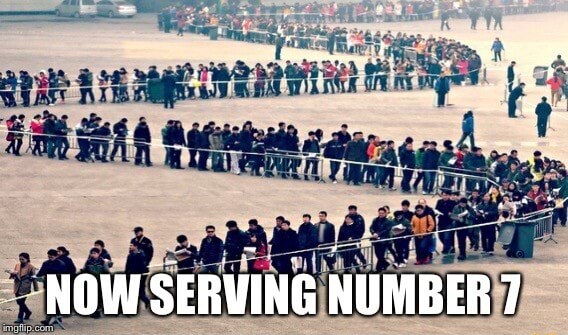
\includegraphics[width=0.6\textwidth]{images/now_serving2}
	\end{center}
\end{frame}

\begin{frame}[fragile]
	\frametitle{Are We There?}

	\begin{multicols}{2}
		\footnotesize
		\textbf{Producer}
		\begin{verbatim}
	 1. [produce item]
	 2. lock( mutex )
	 3. my_turn = p_turn++
	 4. fifo_push( p_fifo, my_full)
	 5. while count == BUFFER_SIZE ||
	 6.       next_p_turn < my_turn
	 7.    cond_wait( my_full, mutex )
	 8. [add item to buffer]
	 9. count++
	10. next_p_turn++
	11. fifo_pop( p_fifo )
	12. if !fifo_is_empty( c_fifo )
	13.    cond_signal(fifo_head(c_fifo))
	14. unlock( mutex )
		\end{verbatim}
		\columnbreak
		\textbf{Consumer}\vspace{-2em}
		\begin{verbatim}
	 1. lock( mutex )
	 2. my_turn = c_turn++
	 3. fifo_push( c_fifo, my_empty )
	 4. while count == 0 ||
	 5.       next_c_turn < my_turn
	 6.    cond_wait( my_empty, mutex )
	 7. [remove item from buffer]
	 8. count--
	 9. next_c_turn++
	10. fifo_pop( c_fifo )
	11. if !fifo_is_empty( p_fifo )
	12.    cond_signal(fifo_head(p_fifo))
	13. unlock( mutex )
	14. [consume item]
		\end{verbatim}
	\end{multicols}
	\vspace{-2em}

	Does this work?
\end{frame}

\end{document}

